\chapter{Lecture 14}

%--- 信息 ----
\begin{center}
    讲师:王立威 \qquad
    课程时间:25.May.27th \qquad 
    笔记:25.June.9th
\end{center}

\bigskip

当我们在进行多方参与的计算时,每方只拿到了输入的一部分,我们希望讨论为了得到计算的结果,通信的代价几何?
\begin{definition}[通信代价]
    我们考虑Boole函数$f: \{0,1\}^n \times \{0,1\}^n \ra \{0,1\}$. 现在要计算$f(x,y)$,且有两方参与者Alice和Bob,但Alice只能看到$x$而Bob只能看到$y$. \textbf{通信代价}(communication complexity)是指最差情况下所需要的通信总比特数,记作$\CC(f)$.
\end{definition}

这里举了一个例子(太过复杂了,之后再相信陈述,请先看当日的录像42min处),最后可以发现,我们需要将$(x,y)$所有可能的取值划分成若干等值矩形,设一共划分了$R$个,那么通信代价有一个下界是$\log_2 R$.

总结成定理就是
\begin{theorem}
    $\CC(f) \ge \log_2 \chi(f)$,其中$\chi(f)$指最优等值矩形划分的矩形个数. 
\end{theorem}

\begin{example}
    对于等值函数$f_\text{Eq}(x,y) = \mathbb{I}_{x=y}$,试求$\chi(f_\text{Eq})$.
\end{example}
\begin{solution}
    也就是要划分单位矩阵$I_{2^n \times 2^n}$. 注意到对角线的元素两两必然不在同一个等值矩形中,所以个数满足$\chi(f_\text{Eq}) \ge 2^n$,推出$\CC(f)\ge n$.
\end{solution}

\begin{example}
    对于函数 
    \[
    f(x,y) = \begin{cases}
    1 &, \text{if} \ x\land y = 0 \\
    0 &, \text{otherwise}
    \end{cases}
    \]

    其中$\land$表示按位与,试求$\chi(f)$的一个下界.
\end{example} 
\begin{solution}
    关注副对角线上的所有元素,会发现对于$x\neq \tilde{x}$,$f(x,\tilde{x})$和$f(x^c, \tilde{x}^c)$不可能同时为1,所以$\chi(f) \ge 2^n$.
\end{solution}

不难察觉,要精确计算$\chi(f)$是很难的,因此往后我们都将重点放在下界的估计上. 下面将$f$的取值矩阵记作$M(f)_{2^n \times 2^n}$ 

\begin{theorem}
    有$\rank(M(f)) \le \chi_1(f) \le \chi(f)$,其中$\chi_1(f)$表示值为1的矩阵块个数. 
\end{theorem}
\begin{proof}
    注意到$\rank(A+B) \le \rank(A) + \rank(B)$即可证明. 
\end{proof}
\begin{corollary}
    $\CC(f) \ge \log_2 \rank(M(f))$
\end{corollary}

事实上,有理论工作已经证明 
\[
\CC(f) \le \text{poly} \log \rank(M(f))
\]

但使用$\chi(f)$去估计得到的是一个下界,该下界不一定可达(例如下图),下一章会介绍一个上界. 


\begin{figure}[H]
    \centering
    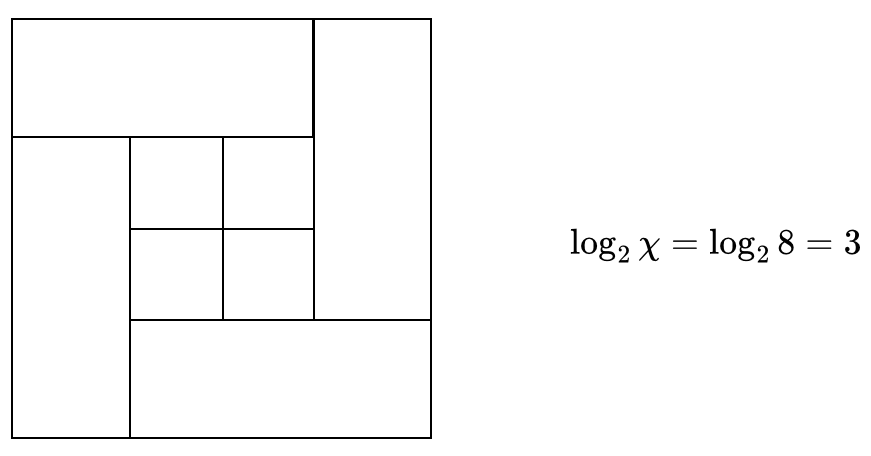
\includegraphics[width=.7\textwidth]{images/c14_1.png}
    \caption{无法达到下界的例子}
\end{figure}